%%========================================================================
%% LaTeX sjabloon voor stage/projectrapport of bachelorproef
%%  HoGent Bedrijf en Organisatie
%%========================================================================

%%========================================================================
%% Preamble
%%========================================================================

\documentclass[pdftex,a4paper,12pt,twoside]{report}

% XXX: Let op: dit sjabloon is gemaakt om dubbelzijdig af te drukken
% Voor enkelzijdig, verwijder ``twoside'' hierboven.

%%---------- Extra functionaliteit ---------------------------------------

\usepackage[utf8]{inputenc}  % Accenten gebruiken in tekst (vb. é ipv \'e)
\usepackage{amsfonts}        % AMS math packages: extra wiskundige
\usepackage{amsmath}         %   symbolen (o.a. getallen-
\usepackage{amssymb}         %   verzamelingen N, R, Z, Q, etc.)
\usepackage[dutch]{babel}    % Taalinstellingen: woordsplitsingen,
                             %  commando's voor speciale karakters
                             %  ("dutch" voor NL)
\usepackage{eurosym}         % Euro-symbool €
\usepackage{geometry}
\usepackage{graphicx}        % Invoegen van tekeningen
\usepackage[pdftex,bookmarks=true]{hyperref}
                             % PDF krijgt klikbare links & verwijzingen,
                             %  inhoudstafel
\usepackage{listings}        % Broncode mooi opmaken
\usepackage{multirow}        % Tekst over verschillende cellen in tabellen
\usepackage{rotating}        % Tabellen en figuren roteren
\usepackage{natbib}          % Betere bibliografiestijlen
\usepackage{fancyhdr}        % Pagina-opmaak met hoofd- en voettekst

\usepackage[T1]{fontenc}     % Ivm lettertypes
\usepackage{lmodern}
\usepackage{textcomp}

\usepackage{lipsum}          % Voor vultekst (lorem ipsum)

%%---------- Layout ------------------------------------------------------

% hoofdingen, enz.
\pagestyle{fancy}
% enkel hoofdstuktitel in hoofding, geen sectietitel (vermijd overlap)
\renewcommand{\sectionmark}[1]{}

% lijn, wordt gebruikt in titelpagina
\newcommand{\HRule}{\rule{\linewidth}{0.5mm}}

% Leeg blad
\newcommand{\emptypage}{
\newpage
\thispagestyle{empty}
\mbox{}
\newpage
}

% Gebruik een schreefloos lettertype ipv het "oubollig" uitziende
% Computer Modern
\renewcommand{\familydefault}{\sfdefault}

% Commando voor invoegen Java-broncodebestanden (dank aan Niels Corneille)
% Gebruik: \codefragment{source/MijnKlasse.java}{Uitleg bij de code}
\newcommand{\codefragment}[2]{ \lstset{%
  language=java,
  breaklines=true,
  float=th,
  caption={#2},
  basicstyle=\scriptsize,
  frame=single,
  extendedchars=\true
}
\lstinputlisting{#1}}

%%---------- Documenteigenschappen ---------------------------------------
%% Vul dit aan met je eigen info:

% Je eigen naam
\newcommand{\student}{Michiel De Wilde}

% De naam van je lector, begeleider, promotor
\newcommand{\promotor}{Bert Van Vreckem}

% De naam van je co-promotor
\newcommand{\copromotor}{Jan Janssen}

% Indien je bachelorproef in opdracht van een bedrijf of organisatie
% geschreven is, geef je hier de naam.
\newcommand{\instelling}{Hogeschool Gent}

% De titel van het rapport/bachelorproef
\newcommand{\titel}{Unikernels}

% Datum van indienen
\newcommand{\datum}{29 mei 2015}

% Faculteit
\newcommand{\faculteit}{Faculteit Bedrijf en Organisatie}

% Soort rapport
\newcommand{\rapporttype}{Scriptie voorgedragen tot het bekomen van de graad van\\Bachelor in de toegepaste informatica}

% Academiejaar
\newcommand{\academiejaar}{2015-2016}

% Examenperiode
%  - 1e semester = 1e examenperiode
%  - 2e semester = 2e examenperiode
%  - tweede zit = 3e examenperiode
\newcommand{\examenperiode}{2e examenperiode}

%%========================================================================
%% Inhoud document
%%========================================================================

\begin{document}

%%---------- Front matter ------------------------------------------------
%% Het voorblad - Hier moet je in principe niets wijzigen.

\begin{titlepage}
  \newgeometry{top=2cm,bottom=1.5cm,left=1.5cm,right=1.5cm}
  \begin{center}

    \begingroup
    \rmfamily
    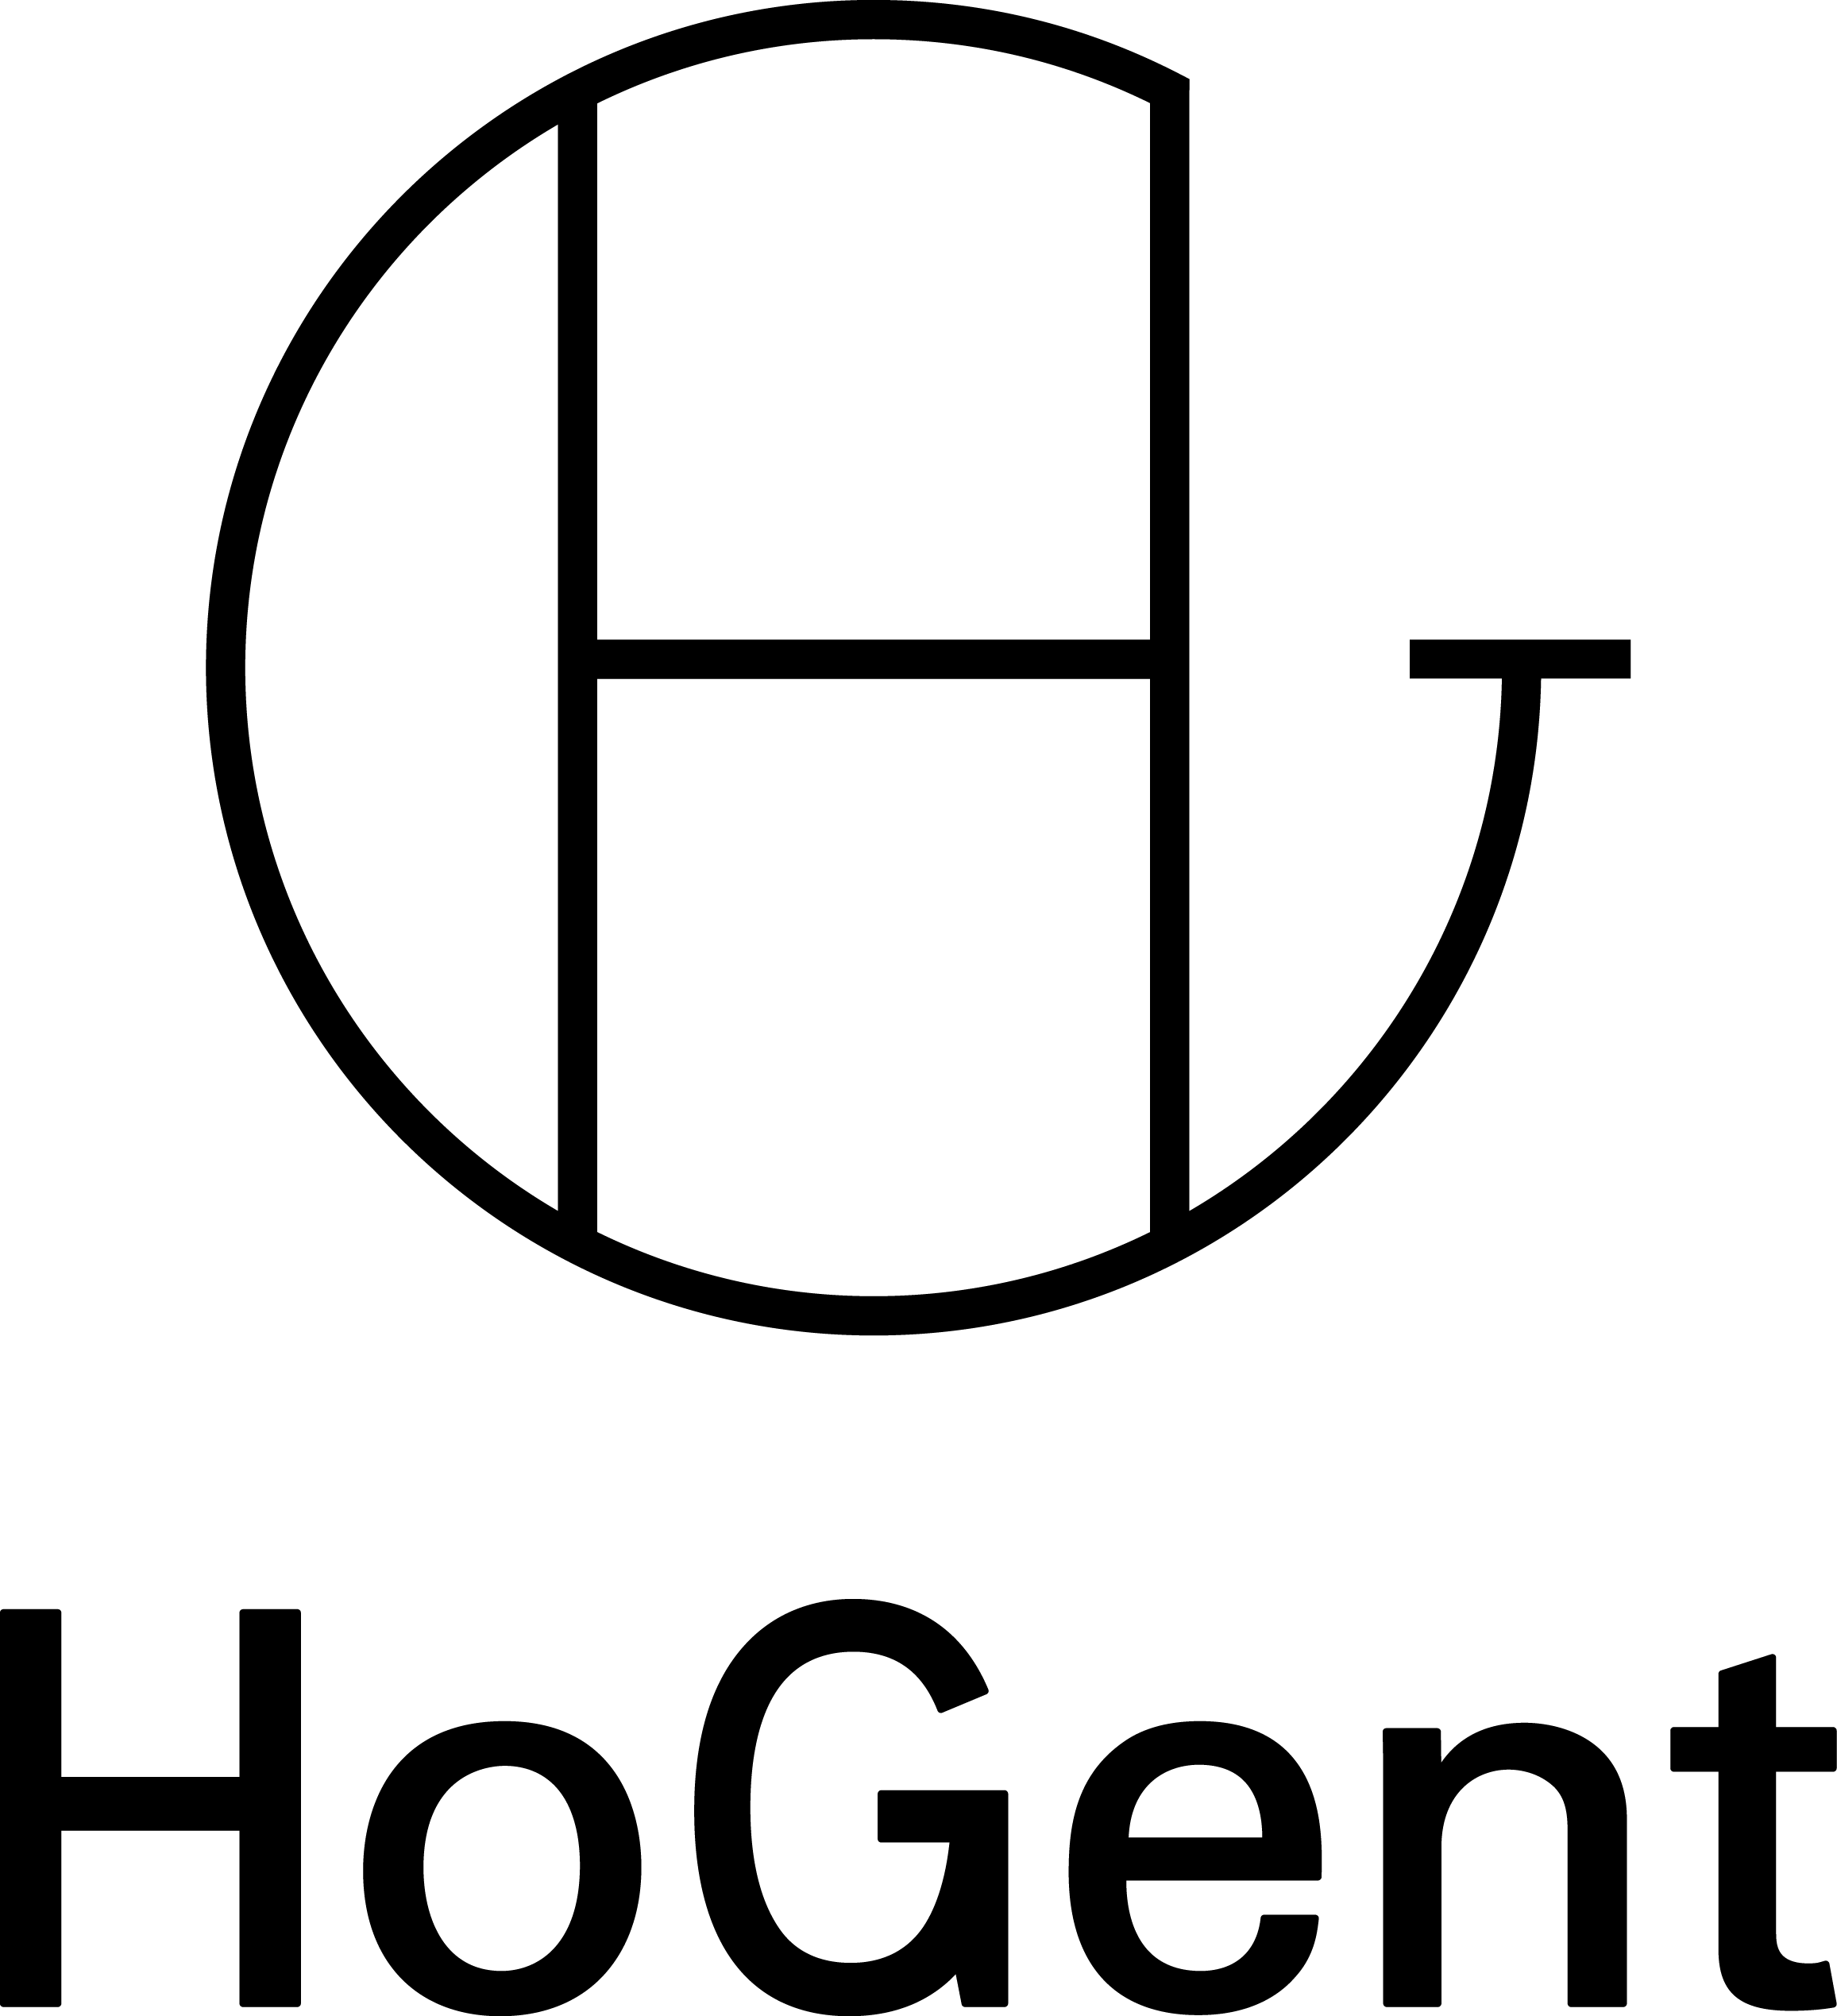
\includegraphics[width=2.5cm]{img/HG-beeldmerk-woordmerk}\\[.5cm]
    \faculteit\\[3cm]
    \titel
    \vfill
    \student\\[3.5cm]
    \rapporttype\\[2cm]
    Promotor:\\
    \promotor\\
    Co-promotor:\\
    \copromotor\\[2.5cm]
    Instelling: \instelling\\[.5cm]
    Academiejaar: \academiejaar\\[.5cm]
    \examenperiode
    \endgroup

  \end{center}
  \restoregeometry
\end{titlepage}

% Schutblad

\emptypage


\begin{titlepage}
  \newgeometry{top=5.35cm,bottom=1.5cm,left=1.5cm,right=1.5cm}
  \begin{center}

    \begingroup
    \rmfamily
    \faculteit\\[3cm]
    \titel
    \vfill
    \student\\[3.5cm]
    \rapporttype\\[2cm]
    Promotor:\\
    \promotor\\
    Co-promotor:\\
    \copromotor\\[2.5cm]
    Instelling: \instelling\\[.5cm]
    Academiejaar: \academiejaar\\[.5cm]
    \examenperiode
    \endgroup

  \end{center}
  \restoregeometry
\end{titlepage}


\begin{abstract}
% TODO: De "abstract" of samenvatting is een kernachtige (max 1 blz. voor een
% thesis) synthese van het document. In ons geval beschrijf je kort de
% probleemstelling en de context, de onderzoeksvragen, de aanpak en de
% resultaten.
  \lipsum[1-4]
\end{abstract}

\chapter*{Voorwoord}
\label{ch:voorwoord}

Toen ik begon met programmeren had ik geen idee wat er gebeurde in de achtergrond van de computer. Ik starte met de simpele todolist-applicaties om alles te leren over programmeren. Na een tijd kwam ik een black box tegen: het besturingssysteem. Vooral om servers sneller te laten werken en de techniek erachter te leren kennen begon ik aan een zoektocht. Linux was de startplek bij uitstek. Package managers en file systems waren de eerste concepten die mij met verstomming lieten staan. Toen ik meer en meer naar infrastructuur keek begon ik termen te leren en alle handige tips om ervoor te zorgen dat je server altijd beschikbaar is. Toen een paar jaar geleden Docker voor het eerst echt vaart maakte met containers was ik verbaasd. Ik dacht eerst dat dit nooit zou werken. Na een tijd heb ik wel het licht gezien en gebruikte ik containers meer en meer. Toen er gevraagd werd om een onderwerp voor mijn thesis dacht ik meteen en wat volgens mij de volgende stap is: unikernels.



\tableofcontents

% Als je een lijst van afkortingen of termen wil toevoegen, dan hoort die
% hier thuis. Gebruik bijvoorbeeld de ``glossaries'' package.

%%---------- Kern --------------------------------------------------------

\chapter{Inleiding}
\label{ch:inleiding}

De wereld is steeds in verandering. Dit is een zekere waarheid in de wereld van informatica. Kijk maar naar de veranderingen dat er gebeuren elke paar maanden op vlak van javascript frameworks. Best practices van vijf jaar geleden, kunnen bad practices zijn vandaag. Je moet mee met de deze stroom van veranderingen wil je relevant blijven. Dit is voor iedereen in uitdaging. In mijn mening is dit iets goed, blijven leren is een van de beste dingen die je kan doen.

Er zijn grote veranderingen aan het gebeuren op het vlak van infrastructuur. Een paar geleden was de een virtuele machine met een klassieke stack de normale gang van zaken. De verandering heeft hier ook voor veranderingen gezorgd. Een container was al een tijd een droom van vele mensen maar er was nog geen echte goede uitwerking. Tot Docker. Met Docker werden containers eenvoudiger om te gebruiken. Unikernels zitten nu in de situatie van containers vooraleer Docker opzetten kwam. Zal unikernels dezelfde revolutie ontketenen of zal het hand in hand kunnen leven met Docker? Docker heeft unikernel systems overgenomen begin vorige jaar en je kan de invloed al zien in hun releases. \\

Deze thesis focust niet enkel op unikernels. 1 Van de onderzoeksvragen gaat over de rol van systeembeheerder in de toekomst. Unikernels en Docker hebben een groot gevolg voor hun maar zijn nog andere factoren die een rol spelen zoals orchestration frameworks, registries, CI/CD en veel meer.

Ik zal mijn uiterste best doen om deze omgeving te beschrijven en aan te tonen wat er kan gebeuren in de toekomst maar er kunnen natuurlijk nieuwe technologieen te voorschijn komen. Dit is een antwoord op de onderzoeksvragen vanuit mijn standpunt en de huidige informatie beschikbaar.

\section{Probleemstelling en Onderzoeksvragen}
\label{sec:onderzoeksvragen}

Unikernels zijn een een nieuwe stroom binnen het landschap van besturingssystemen. We hebben al aangehaald dat containers de nieuwe werkwijze is wanneer men applicaties wilt ontwikkelen en schaalbaar wilt maken. Unikernels gaat nog een stap verder. De systeembeheerders moeten dus mee met containers en de veranderingen ondergaan. De vraag is welke veranderingen er zich zullen voordoen wanneer unikernels op de markt komen. Zullen de competenties van de systeembeheerder veranderen? Wordt het opzetten van applicaties meer en meer eenvoudiger of juist niet? We kunnen wel spreken over de opvolger van containers maar is deze al werkbaar in de toekomst? Wat is de impact op beveiliging, meer bepaald aspecten als beschikbaarheid, autorisatie, integriteit en vertrouwelijkheid van gegevens?


\chapter{Methodologie}
\label{ch:methodologie}

% TODO: Hoe ben je te werk gegaan? Verdeel je onderzoek in grote fasen, en
% licht in elke fase toe welke stappen je gevolgd hebt. Verantwoord waarom je
% op deze manier te werk gegaan bent. Je moet kunnen aantonen dat je de best
% mogelijke manier toegepast hebt om een antwoord te vinden op de
% onderzoeksvraag.

\chapter{Virtualisatie}
\label{ch:virtualisatie}

Vroeger was de tijd dat je een computer kon gebruiken beperkt. Vooral bij de eerste computers had men problemen om programma's en concepten uit te werken omdat de computer door meerdere mensen gebruikt werd. Een voorbeeld vanuit een situatie uit die tijd is het ontwikkelen van een programma. De source code van een programma werd manueel ingegeven en als een job in een queue gezet. Pas een paar dagen later kon men de resultaten bekijken. Als je een kleine schrijf- en/of logische denkfout maakte dan kon je opnieuw beginnen. De grootste bijdrage tot de ontwikkelsnelheid van programma's is de lengte van de feedbackcyclus: hoe snel kan je je programma testen laten werken. Dit leidt tot een verlies van tijd en dus geld.

Timesharing werd uitgevonden om het verlies van tijd te beperken. Bij timesharing konden de gebruikers inloggen op een console en zo computer gebruiken. Dit was een technische uitdaging. De computer zou van de ene context naar de andere moeten kunnen veranderen. Timesharing en verschillende gebruikers op 1 computer zou de basis vormen voor de moderne besturingsystemen. 1 Van de nadelen van timesharing is de isolatie van twee verschiilende processen. Als er een kans bestaat dat ze elkaar kunnen beinvloeden is dit een heel groot probleem.

Een besturingsysteem moet kunnen werken op verschillende soorten hardware. Om al deze hardware te ondersteunen moet er een standaard zijn waarop een besturingssysteem kan gebouwd worden. Dit zou betekenen dat veel van de complexiteit van het besturingssysteem naar de hardware zou verhuizen. Spijtig genoeg gebeurt dit nog altijd niet. Dit is 1 van de voornaamste redenen waarom de grootte van een OS tussen de 200MB en 1GB kan liggen. Een aantal besturingssystemen doen niet de moeite om de vele soorten hardware apparatuur te ondersteunen. Zij tonen de specificaties die een hardware apparaat moet hebben wanneer je het besturingssysteem wil gebruiken. \newpage

Doorheen de tijd werden computers meer krachtig en applicaties konden niet alle middelen van de computer ten volle benutten. Dit zorgde voor de creatie van virtual resources. Deze gingen de fysieke hardware simuleren om zo verschillende applicaties tegelijkertijd te laten werken op dezelfde virtuele machine. Zo worden de middelen van een fysieke machine optimaal gebruikt. De algemene term voor dit concept is virtualisatie. Bij het virtualiseren van een server gaat men een fysieke server opdelen in verschillende kleine en geisoleerde delen. Deze delen kunnen dan gebruikt worden door verschillende gebruikers. De voordelen van het virtualiseren van een server zijn de volgende: financieel voordeel (men kan van 1 taak naar meerdere taken gaan op 1 server), het besparen van energie (minder servers gebruiken want ze worden beter benut), betere beschikbaarheid.

\section{Hypervisor}

Een hypervisor is een stuk software, firmware of hardware waarop een virtuele machine zich bevindt. De host machine zorgt voor de middelen zoals CPU, RAM, ... Elke virtuele machine die zich bevindt op de host machine zal dan gebruik maken van deze middelen. Doordat virtualisatie alomtegenwoordig werd in datacenters heeft het ervoor gezorgd dat de meeste logica ook meer kwam te liggen bij de hypervisor. Cloud computing komt zeer sterk opzetten en dit zorgt ervoor dat de meeste mensen niet in contact komen met hypervisors.

\subsection{Hosted Hypervisors}

Een hosted hypervisor zal zich bevinden op een het besturingssysteem van de host machine en heeft geen directe toegang tot de hardware. Dit heeft als voordeel dat de hardware niet zo belangrijk is maar zorgt voor een extra laag tussen de hardware en de hypervisor. Een goede regel is: "hoe minder lagen we hebben, hoe beter de performantie." Wanneer je een Ubuntu instantie hebt in een virtuele machine dan zal de computer de hypervisor zijn. De computer kan dan de virtuele machine beheren en veranderingen uitvoeren.

Voorbeelden van een hosted hypervisor zijn: Virtualbox en VMware Workstation.

\subsection{Bare-metal Hypervisors}

Een alternatief is een bare-metal hypervisor. Hierbij is er geen extra laag tussen de hardware en de virtuele machine. We hebben geen host besturingssysteem nodig omdat de hypervisor zich rechtstreeks bevindt op de hardware. Dit zorgt voor betere performantie, schaalbaarheid en stabiliteit. Het wordt ook gebruikt in bijna alle  \\

\section{Hardware Virtualization}

De virtuele machine is een toepassing van de virtualisatie van de hardware. Een virtuele machine bevindt zich op een fysieke machine door gebruik te maken van een hypervisor. De nadelen van een virtuele machine als de kleinste eenheid is de schaalbaarheid en de veiligheid. Wanneer je je eigen server opstelde dan moet je een besturingssysteem kiezen. Meestal gaan we kiezen voor een Linux distributie. Daarna moet je de software installeren die ervoor zorgt dat de applicatie kan werken. Daaropvolgend moet je je server beveiligen. Het veranderen van de SSH-poort, zorgen dat de root-user niet te bereiken is. IPtables en firewalls opstellen. Voor dit te vergemakkelijken kunnen we gebruikmaken van een configuratie management tool (Chef, Puppet, Ansible...).

Meest bekende voorbeelden van bare-metal hypervisors zijn VMware ESXi, Microsoft Hyper-V en Xen.

\section{Operating System-level Virtualization}

Naast hardware virtualisatie kunnen we ook gebruikmaken van de virtualisatie van het besturingssysteem. Bij deze toepassing van virtualisatie gaan we de mogelijkheden van de kernel van het besturingssysteem gebruiken. De kernel van bepaalde besturingssystemen laat ons toe om meerdere geisoleerde user spaces tegelijkertijd te laten werken. Dit zorgt ervoor dat de dat er maar 1 besturingssysteem en een kernel zijn. De verschillende user spaces maken gebruik van CPU, geheugen en netwerk van de host server. Elke user space heeft zijn eigen configuratie omdat de user spaces op zichzelf staan en geisoleerd zijn de andere user spaces. Tegenover hardware virtualisatie zal de besturingssysteem virtualisatie minder gebruik maken van het geheugen en de CPU omdat er maar 1 kernel is en niet meerdere besturingssystemen. Het opstarten neemt maar een fractie van de tijd in beslag tegenover virtuele machines. Deze user spaces worden ook wel containers genoemd. 

Containers hebben aan populariteit gewonnen door Docker. Docker heeft gezorgd voor ecosysteem, waarbij je gemakkelijk kan starten met containers te gebruiken. 
We starten met het maken van een DockerFile waar we de base-image definieren en wat we verder willen aanpassen. Deze DockerFiles kunnen gedeeld worden en zorgen steeds voor dezelfde uitkomst wanneer je van de DockerFile een image zou maken. Deze image kunnen we dan uitvoeren en dan hebben we een werkende container.
Dockerhub versnelt dit proces in grote mate door DockerFile open te stellen in repositories. Als je bijvoorbeeld een nginx container nodig hebt, dan zoek je voor nginx en neem je versie die jij nodig hebt. De meest gebruikte repositories hebben documentatie hoe je deze container moet gebruiken en hoe je andere containers met elkaar moet verbinden. 

Meest bekende voorbeelden zijn Docker en Rocket.

Er werd al aangehaald bij de virtuele machines dat veiligheid een probleem kan zijn. Dit probleem verdwijnt niet bij containers omdat ze 1 kernel delen. Wanneer de beveiliging van 1 container kan geschonden worden dan wordt het direct gemakkelijker om toegang te verschaffen tot de andere containers. Het gebruiken van 1 OS als de basis voor een aantal containers kan ervoor zorgen dat wanneer dit besturingssysteem niet meer opstaat al deze applicaties niet meer werken.

\chapter{Unikernels}
\label{ch:unikernels}

\section{Inleiding}

Als je stilstaat bij hoe complex een computer is dan zul je beseffen dat het een wonder is dat alles eigenlijk werkt.
Een applicatie doorloopt verschillende stadia om te beginnen werken. De eerste fase is het compileren of interpreteren van de code dat er geschreven is.
Deze zal bepaalde systeem APIs aan roepen van je besturingssysteem.
Deze APIs bevinden zich op een besturingssysteem, die zich dan weer bevindt op een virtuele machine.
Er zijn nog meer lagen die zich tussen de applicatie en de hardware bevinde.
Zoals we al eerder hebben aangehaald is het aantal lagen tussen een applicatie en de hardware 1 van de grootste redenen voor de snelheid van een applicatie.

Wanneer we kijken om iets gemakkelijker te maken of de performantie te verbeteren moeten we kijken naar alle delen. De hardware wordt al meer efficient door gebruik te maken van een hypervisor. Het verschil in de interfaces die de hardware openstellen wordt hierdoor al verminderd. Hypervisors zijn battle-tested. Alle grote cloud providers maken gebruik van hypervisor met succes. Een ander deel dat kan intrigeren is het besturingssysteem. Een besturingssysteem waarop een applicatie bevindt is in de meeste gevallen een Linux besturingssysteem. 1 Van de meest bekende besturingssystemen voor servers is Ubuntu. Het lijkt raar dat een besturingssysteem dat zich wil openstellen aan het grote publiek ook gebruikt wordt voor servers. Sommige delen van een besturingssysteem zijn ook niet meer nodig. We hebben het eerder al gehad over een deel dat misschien niet thuishoort op servers: time-sharing. Time-sharing zorgt ervoor dat de systeem en hardware componenten van de gebruiker worden afgeschermd. Een gebruiker die een programma liet werken zou een andere programma gestart door een andere gebruiker kunnen laten stoppen door een bepaalde instructie uit te voeren. Dit probleem is bijna niet meer voorkomend doordat hardware zou goedkoop is geworden en iedereen zijn eigen computer heeft.

Niet alleen hebben sommige delen quasi geen nut meer maar sommige delen zullen ervoor zorgen dat de performantie van een server gehinderd wordt voor bepaalde taken. Het is dezelfde analogie als het gebruiken van een hamer voor alle klusjes die je moet doen. Het is niet omdat een hamer goed is voor bepaalde taken dat het goed is voor alles. Dit probleem kunnen we zeker bezien door te bekijken hoeveel besturingssystemen zijn veranderd doorheen de laatste 20 jaar. Er zijn zoveel veranderingen op het vlak van computing dat het raar lijkt dat sommige delen perfect blijven. 

Soms kan starten met blanke pagina ervoor zorgen dat er een betere oplossing gevonden wordt. Wanneer we blijven denken met besturingssysteem dan zal de oplossing een variant van een besturingssysteem zijn. Het weggooien van het concept van een besturingssysteem voor servers lijkt radicaal maar kan het veel slechter zijn dan de huidige situatie? 

Het programmeren van al de system calls die we nodig hebben om een applicatie te laten werken is veel werken. Maar we moeten niet al de functionaliteit van een besturingssysteem uitwerken. Het laten van werken van een 1 applicatie systeem is veel gemakkelijker te implementeren dan een systeem voor een 1 gebruiker.

Ik heb al aangehaald dat we besturingssystemen gebruikten, als de provisoning unit op onze servers. Nadat ik al de nadelen van de huidige besturingssystemen heb laten zien, kun je wel opmaken dat dit misschien geen goed idee is. 1 Van de voordelen van deze aanpak is dat we besturingssystemen al kennen omdat we er elke dag met werken. Als we een ander concept introduceren dan zou het veel meer moeite zijn om uw infrasstructuur te laten werken. We verloren wel een deel van onze performantie.

De reactie op het verspillen van deze resources was de container. Docker zorgde voor een gemakkelijke gebruikerservaring om containers te gebruiken en dit zorgde voor een revolutie binnen devops. Het nadeel van containers is de veiligheid. Er zijn veel voorbeelden van containers die niet optimaal van elkaar gescheiden zijn.

Daar is waar unikernels te voorschijn komen. Waarom zou je je applicaties niet :rechtstreeks op de hypervisor kunnen laten werken? De hypervisor zorgt voor een interface en de unikernels zal de nodige functionaliteit implementeren. Dit zorgt ervoor dat elke applicatie afzonderlijk kan worden geoptimaliseerd. De hypervisor kan zelf bepalen hoeveel geheugen of CPU een bepaalde applicatie nodig heeft.

Op DockerHub kan veel images van bepaalde containers vinden. Er zijn gespecialiseerde containers voor Golang met minimale besturingssystemen en deze images bestaan uit meerdere layers. Je kan dus layers maken die kunnen hergebruikt worden voor verschillende images. Bij unikernels gaan we functionaliteit splitsen in drivers. Het zou gemakkelijk moeten zijn voor drivers te gebruiken in jouw applicatie.


\chapter{Conclusie}
\label{ch:conclusie}

% TODO: Trek een duidelijke conclusie, in de vorm van een antwoord op de
% onderzoeksvra(a)g(en). Reflecteer kritisch over het resultaat. Zijn er
% zaken die nog niet duidelijk zijn? Heeft het ondezoek geleid tot nieuwe
% vragen die uitnodigen tot verder onderzoek?


\bibliographystyle{apa}
\bibliography{tin-bachproef}

%%---------- Back matter -------------------------------------------------

\listoffigures
\listoftables

\end{document}
